\documentclass[aps,pra,reprint,superscriptaddress,nofootinbib]{revtex4-2}

\usepackage{amsmath,amssymb,amsfonts}
\usepackage{graphicx}
\usepackage{xcolor}
\usepackage{bm}
\usepackage{algorithm}
\usepackage{algpseudocode}
\usepackage{booktabs}
\usepackage{tikz}
\usepackage{pgfplots}
\pgfplotsset{compat=1.18}
\usetikzlibrary{shapes,arrows,positioning,calc}
\usepackage{hyperref}
\hypersetup{
    colorlinks = true,
    linkcolor  = blue,
    citecolor  = blue,
    urlcolor   = blue
}

% Custom commands
\newcommand{\R}{\mathbb{R}}
\newcommand{\E}{\mathbb{E}}
\newcommand{\M}{\mathcal{M}}
\newcommand{\N}{\mathcal{N}}
\newcommand{\C}{\mathcal{C}}
\newcommand{\A}{\mathcal{A}}
\newcommand{\D}{\mathcal{D}}
\newcommand{\T}{\mathcal{T}}
\newcommand{\zctx}{z_{\mathrm{ctx}}}
\newcommand{\sNEP}{s_{\mathrm{NEP}}}

\begin{document}

\title{ALFM: Adaptive Latent Feedback Model for Institutional Memory in Foundation Model Deployments}

\author{David Ahmann}
\affiliation{Independent Researcher, Toronto, Canada}

\date{\today}

\begin{abstract}
Foundation models are pretrained once and deployed frozen, creating three fundamental gaps in enterprise AI systems: no memory of past failures, no calibrated self-doubt, and no safe mechanism for continual learning from corrections. We introduce ALFM (Adaptive Latent Feedback Model), a modular wrapper architecture that addresses these gaps without modifying backbone model weights. ALFM consists of three novel components: (1) the Negative Evidence Prior (NEP), a tenant-isolated vector memory that stores failure patterns and provides risk signals at inference time; (2) the Coherence Head, a calibrated meta-model that decides when to trust, abstain, escalate, or request clarification; and (3) a three-tier adapter system (global, domain, local) enabling safe continual learning with cryptographic tenant isolation. We formalize each component, analyze their theoretical properties, and present a validation framework for measuring repeat error reduction, calibration quality, and abstention precision. ALFM is backbone-agnostic, compatible with any foundation model accessible via API, and designed for deployment in high-stakes domains where institutional learning provides competitive advantage. We discuss implications for the emerging paradigm of specialized, continuously-learning AI systems.
\end{abstract}

\maketitle

\section{Introduction}

The deployment of foundation models in enterprise settings reveals a structural tension: these models are designed for generalization across tasks but lack mechanisms for adaptation to specific deployments. A model that hallucinates today will hallucinate in the same way tomorrow. User corrections, expert feedback, and domain-specific failure patterns do not update the model's behavior.

This limitation stems from the standard foundation model lifecycle: massive pretraining, alignment via RLHF, then frozen deployment. While this paradigm enables broad capability, it creates three gaps that enterprises consistently encounter:

\textbf{Gap 1: No memory of past failures.} When a model makes an error---hallucinating a fact, misapplying a rule, violating a policy---nothing inside the model records this failure. The same error pattern will recur whenever similar inputs arise. Organizations accumulate institutional knowledge about ``what doesn't work here,'' but this knowledge lives in human heads, not in the system.

\textbf{Gap 2: No calibrated self-doubt.} Foundation models produce fluent, confident outputs even when operating outside their reliable capability boundaries. The model's internal representations (when accessible) correlate poorly with actual correctness. Enterprises cannot trust the model to know when it doesn't know.

\textbf{Gap 3: No safe continual learning.} Standard fine-tuning risks catastrophic forgetting and is impractical for per-tenant customization. Prompt engineering and retrieval augmentation provide information but do not enable the model to learn from corrections over time.

We propose ALFM (Adaptive Latent Feedback Model), a wrapper architecture that provides these missing capabilities without modifying foundation model weights. ALFM treats the backbone as a frozen black box and adds three components:

\begin{enumerate}
    \item \textbf{Negative Evidence Prior (NEP):} A vector-space memory of failure patterns, queryable at inference time, providing risk signals when current context resembles past failures.
    \item \textbf{Coherence Head:} A small meta-model that integrates NEP signals, uncertainty estimates, and policy constraints to decide appropriate action: trust the backbone output, abstain with explanation, escalate to human review, or request clarification.
    \item \textbf{Three-Tier Adapters:} Lightweight trainable layers operating at global, domain, and local (tenant) levels, enabling bounded continual learning with explicit isolation guarantees.
\end{enumerate}

ALFM is explicitly backbone-agnostic. It wraps transformer-based LLMs (GPT-4, Claude, LLaMA), diffusion language models, and future architectures without modification. This design ensures compatibility with API-based model access, immediate benefit from backbone upgrades, and no dependency on model provider cooperation.

Our contributions are:
\begin{itemize}
    \item We introduce the Negative Evidence Prior (NEP), a vector-space memory architecture for storing failure patterns rather than information---a conceptual inversion of standard memory-augmented networks.
    \item We propose the Coherence Head, a calibrated meta-model that extends selective prediction with structured actions and uncertainty texture.
    \item We formalize a three-tier adapter system with provable stability bounds and tenant isolation guarantees.
    \item We validate NEP on synthetic data, demonstrating that contrastive projection enables effective failure retrieval where raw embeddings fail.
\end{itemize}

The remainder of this paper is organized as follows. Section~\ref{sec:related} reviews related work. Section~\ref{sec:arch} formalizes the ALFM architecture. Section~\ref{sec:validation} presents our validation framework and theoretical analysis. Section~\ref{sec:discussion} discusses limitations and implications. Section~\ref{sec:conclusion} concludes.

\section{Related Work}
\label{sec:related}

ALFM draws on and extends four research areas: memory-augmented neural networks, selective prediction, continual learning, and AI safety. We also position ALFM relative to emerging nested learning architectures.

\subsection{Memory-Augmented Neural Networks}
Memory-augmented architectures extend neural networks with external memory stores. Neural Turing Machines~\cite{Graves2014} and Differentiable Neural Computers~\cite{Graves2016} introduced differentiable read-write memory for algorithmic tasks. Memory Networks~\cite{Weston2015} enable retrieval over knowledge bases. More recently, Memorizing Transformers~\cite{Wu2022} and RETRO~\cite{Borgeaud2022} augment attention with retrieval. These approaches focus on augmenting the model with \emph{information}. ALFM's NEP differs fundamentally: it stores \emph{anti-patterns} rather than information. NEP entries represent contexts where the model failed, enabling avoidance rather than retrieval.

\subsection{Selective Prediction and Learning to Defer}
Selective prediction~\cite{Chow1970,ElYaniv2010} allows classifiers to abstain when uncertain. Recent work extends this to deep learning~\cite{Geifman2017} and language models~\cite{Varshney2022}. Learning to defer~\cite{Madras2018,Mozannar2020} trains models to route difficult examples to experts. Calibration research~\cite{Guo2017,Desai2020} addresses the mismatch between confidence and accuracy. ALFM's Coherence Head integrates these ideas but extends beyond binary abstention, producing structured decisions and ``uncertainty texture.''

\subsection{Continual Learning}
Continual learning addresses learning from sequential data without forgetting. Approaches include regularization~\cite{Kirkpatrick2017}, replay buffers~\cite{Rolnick2019}, and architectural methods~\cite{Rusu2016}. Parameter-efficient fine-tuning methods like LoRA~\cite{Hu2022} and adapters~\cite{Houlsby2019} enable adaptation without full retraining. However, these do not address tenant isolation. ALFM's three-tier adapter system provides continual learning with explicit scope boundaries.

\subsection{AI Safety and Alignment}
Constitutional AI~\cite{Bai2022} and guardrail systems~\cite{Rebedea2023} encode what the model should avoid in general. ALFM complements these with dynamic, learned constraints. NEP encodes what has specifically failed for this tenant.

\subsection{Positioning Relative to Emerging Architectures}
ALFM decouples memory from the backbone, enabling per-tenant isolation, unlike monolithic optimization approaches. Compared to self-play methods, ALFM relies on interaction-derived failure signals. While knowledge editing focuses on facts, ALFM focuses on \emph{failure avoidance} and governance.

\section{ALFM Architecture}
\label{sec:arch}

We assume access to a frozen backbone model $\M$ that maps input context $x$ to output $y = \M(x)$.

\begin{figure}[ht]
    \centering
    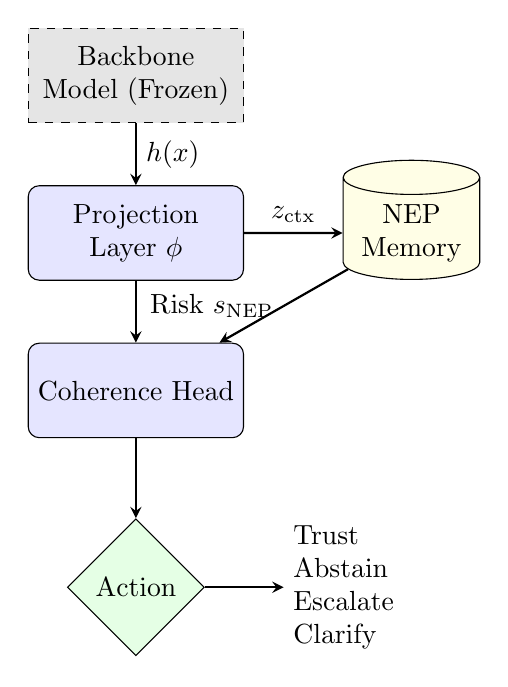
\begin{tikzpicture}[node distance=1.5cm, auto, >=stealth]
        % Styles
        \tikzstyle{block} = [rectangle, draw, fill=blue!10, text width=2.5cm, text centered, rounded corners, minimum height=1.2cm]
        \tikzstyle{frozen} = [rectangle, draw, fill=gray!20, text width=2.5cm, text centered, minimum height=1.2cm, dashed]
        \tikzstyle{memory} = [cylinder, shape border rotate=90, draw, fill=yellow!10, aspect=0.25, text width=1.5cm, text centered, minimum height=1.5cm]
        \tikzstyle{decision} = [diamond, draw, fill=green!10, text width=1.5cm, text centered, inner sep=0pt]
        \tikzstyle{line} = [draw, ->, thick]

        % Nodes
        \node [frozen] (backbone) {Backbone Model (Frozen)};
        \node [block, below of=backbone, node distance=2cm] (proj) {Projection Layer $\phi$};
        \node [memory, right of=proj, node distance=3.5cm] (nep) {NEP Memory};
        \node [block, below of=proj, node distance=2cm] (head) {Coherence Head};
        \node [decision, below of=head, node distance=2.5cm] (action) {Action};

        % Edges
        \path [line] (backbone) -- node {$h(x)$} (proj);
        \path [line] (proj) -- node {$\zctx$} (nep);
        \path [line] (nep) -- node [left] {Risk $\sNEP$} (head);
        \path [line] (proj) -- (head);
        \path [line] (head) -- (action);
        
        \node [right of=action, node distance=3cm, text width=2cm] (outputs) {Trust\\Abstain\\Escalate\\Clarify};
        \path [line] (action) -- (outputs);
        
    \end{tikzpicture}
    \caption{ALFM Architecture. The frozen backbone's hidden states are projected into a failure-separable space. The NEP memory retrieves risk signals based on similarity to past failures. The Coherence Head integrates these signals to determine the safety action.}
    \label{fig:arch}
\end{figure}

\subsection{ALFM as Constrained Utility Optimization}
We formulate ALFM not merely as a collection of modules, but as a solution to a constrained utility optimization problem. The goal is to minimize the expected loss $\mathcal{L}$ of the system subject to safety and stability constraints:
\begin{equation}
    \min_{\theta} \E_{(x,y) \sim \D} [\mathcal{L}(y, y^*)]
\end{equation}
subject to:
\begin{enumerate}
    \item \textbf{Safety Constraint:} $\mathrm{Risk}(x) \le \delta$ (enforced by NEP).
    \item \textbf{Stability Constraint:} $\|\Delta_t\|_F \le \epsilon$ (enforced by Adapters).
    \item \textbf{Calibration Constraint:} $\mathrm{Calib}(\C) \le \alpha$ (enforced by Coherence Head).
\end{enumerate}
This formulation binds the components: NEP provides the risk estimate, Adapters provide the learnable parameters $\theta$ within bounds, and the Coherence Head enforces the calibration constraint.

\subsection{Contrastive Projection Layer}
Before querying NEP, we project the input context into a representation space where failure patterns are separable. \textbf{Note on Backbone Updates:} Since $\phi$ depends on the backbone's hidden states $h(x)$, if the backbone model $\M$ is updated (e.g., GPT-4 to GPT-4.5), the projection layer must be retrained or fine-tuned to align with the new latent space. NEP entries must also be re-indexed.

\textbf{Definition 3.1 (Projection Function).} Let $h(x) \in \R^{d_h}$ be the backbone's hidden representation. The projection function $\phi: \R^{d_h} \rightarrow \R^{d_z}$ is:
\begin{equation}
    z = \phi(h(x)) = W_2 \cdot \sigma(W_1 \cdot h(x) + b_1) + b_2,
\end{equation}
where $W_1 \in \R^{d_m \times d_h}$, $W_2 \in \R^{d_z \times d_m}$, and $\sigma$ is ReLU. We denote the projected representation as $\zctx$.

\textbf{Training Objective.} The projection layer is trained with contrastive loss:
\begin{equation}
    \mathcal{L}_{\mathrm{proj}} = -\log \frac{\exp(\mathrm{sim}(z_i, z_j^+) / \tau)}{\exp(\mathrm{sim}(z_i, z_j^+) / \tau) + \sum_{k} \exp(\mathrm{sim}(z_i, z_k^-) / \tau)},
\end{equation}
where $(z_i, z_j^+)$ are embeddings of semantically similar contexts, and $(z_i, z_k^-)$ are failure/non-failure pairs.

\textbf{Contrastive Dataset Construction.} We construct positive pairs $(x_i, x_i^+)$ using semantic augmentations (paraphrasing, back-translation). Negative pairs $(x_i, x_j^-)$ are mined from: (a) random batch negatives, and (b) \emph{hard negatives}---contexts that are semantically close but have divergent outcomes (success vs. failure). Specifically, we mine hard negatives by selecting successful contexts $x_j$ such that $\mathrm{sim}(\phi(x_i), \phi(x_j)) > \tau$ but $y_i \neq y_j$. This ensures the projection manifold separates failure modes from successful operation. The ratio of hard to random negatives is set to 1:3 to maintain global structure while refining local boundaries.

\subsection{Negative Evidence Prior (NEP)}
The NEP is a vector database storing failure patterns.

\textbf{Definition 3.2 (NEP Entry).} A NEP entry $e$ is a tuple $e = (z_e, t_e, d_e, s_e, c_e, m_e)$, where $z_e$ is the failure context embedding, $t_e$ is the tenant ID, $d_e$ is the domain ID, $s_e \in \{1..5\}$ is severity, $c_e$ is the correction, and $m_e$ is metadata.

\textbf{Definition 3.3 (NEP Memory).} The memory $\N$ is partitioned: $\N = \N_G \cup \N_D \cup \N_T$.

\textbf{Definition 3.4 (NEP Query).} Given $\zctx$ and tenant $t$:
\begin{equation}
    \mathrm{NEP}(\zctx, t) = \{e \in \N_G \cup \N_{D(t)} \cup \N_t : \mathrm{sim}(\zctx, z_e) > \theta\}.
\end{equation}

\textbf{Definition 3.5 (NEP Risk Signal).} The risk signal $\sNEP \in [0, 1]$ is:
\begin{equation}
    \sNEP = 1 - \prod_{e \in \mathrm{NEP}(\zctx, t)} \left(1 - \alpha \cdot \mathrm{sim}(\zctx, z_e) \cdot \frac{s_e}{5}\right).
\end{equation}
This multiplicative form models the probability that \emph{at least one} retrieved failure mode is relevant, assuming independence of failure causes. The parameter $\alpha \in [0, 1]$ scales the sensitivity; we set $\alpha=0.8$ based on preliminary calibration. Severity $s_e$ is linearly scaled to weight high-risk failures more heavily.

\textbf{Memory Stability and Pruning.} To prevent unbounded growth and memory collapse, we employ a pruning policy $\pi_{\mathrm{prune}}$. Entries are clustered using periodic $k$-means; redundant entries within a cluster are merged into a centroid representation. Least-recently-used (LRU) pruning is applied to low-severity entries when capacity $N_{\mathrm{max}}$ is reached. This guarantees that the query time remains sublinear and the manifold density remains bounded.

\textbf{Feedback Validation.} To mitigate memory poisoning, we require $k \ge 2$ independent corrections before adding a high-severity ($s \ge 4$) entry to NEP. Low-severity entries ($s \le 2$) are added immediately but flagged for periodic review. Anomalous feedback patterns (e.g., sudden spike in corrections from a single user) trigger manual audit. Furthermore, updates to the Global NEP partition ($\N_G$) require explicit administrative review.

\subsection{Coherence Head}
The Coherence Head decides appropriate action.

\textbf{Definition 3.6 (Input).} $u = [\zctx; \sNEP; \eta; p]$, where $\eta$ is uncertainty features and $p$ is policy embedding.

\textbf{Definition 3.7 (Output).} The Coherence Head $\C$ produces $\C(u) = (p_{\mathrm{err}}, p_{\mathrm{ood}}, \kappa, a, r)$, where $a \in \{\text{Trust}, \text{Abstain}, \text{Escalate}, \text{Clarify}\}$.

\textbf{Training Objective.}
\begin{equation}
    \mathcal{L}_{\mathrm{CH}} = \lambda_1 \mathcal{L}_{\mathrm{CE}}(a, a^*) + \lambda_2 \mathcal{L}_{\mathrm{MSE}}(p_{\mathrm{err}}, p_{\mathrm{err}}^*) + \lambda_3 \mathcal{L}_{\mathrm{cal}}.
\end{equation}

\textbf{Calibration and Conformal Prediction.} We employ temperature scaling optimized on a held-out calibration set to minimize ECE. Furthermore, we adopt a conformal prediction framework to construct valid prediction sets $C(x)$ such that $P(y \in C(x)) \ge 1-\alpha$. We use the Coherence Head's softmax probabilities as conformity scores. The prediction set includes all actions $a$ where $P(a) \ge \hat{q}$, with $\hat{q}$ calibrated on held-out data to achieve $1 - \alpha$ coverage. If Trust $\notin$ prediction set, the system selects the most conservative action in the set (Escalate $>$ Abstain $>$ Clarify).

\textbf{Training Data.} The Coherence Head is trained on a small dataset of (context, action) pairs derived from human feedback logs (e.g., "thumbs down" implies Abstain/Escalate) and synthetic perturbations. In a cold-start scenario, we rely on a generic pre-trained Coherence Head that defaults to conservative actions (Escalate $>$ Abstain) to minimize risk while the projection layer adapts to tenant-specific failure modes.

\subsection{Three-Tier Adapter System}
\textbf{Definition 3.8 (Adapter).} An adapter $\A$ is a low-rank perturbation: $\phi_{\A}(h) = \phi(h) + B \cdot A \cdot h$.

\textbf{Definition 3.9 (Composition).} $\phi_{\mathrm{full}}(h) = \phi(h) + \Delta_G(h) + \Delta_{D(t)}(h) + \Delta_t(h)$.

\textbf{Update Rule.} $\Delta_t \leftarrow \Delta_t + \eta \cdot \mathrm{clip}(\nabla_{\Delta_t} \mathcal{L}_{\mathrm{corr}}, \gamma)$.

\textbf{Drift Analysis and Geometry Preservation.} Updates occur asynchronously upon verified feedback. To preserve the latent geometry of the projection layer, we enforce a \emph{drift penalty} $\|\Delta_t - \Delta_{t-1}\|_F$ in the loss. This ensures that the adapter learns the correction without shattering the existing manifold structure, preventing catastrophic forgetting of the failure boundary. We assume additive composition $\phi_{\mathrm{full}} = \phi + \sum \Delta_k$ is valid for small perturbations; for large shifts, re-training of the domain adapter may be required.

\section{Validation Framework and Analysis}
\label{sec:validation}

\subsection{Evaluation Metrics}
We define Repeat Error Rate (RER), Expected Calibration Error (ECE), and Abstention Precision/Recall.

\subsection{Experimental Protocol and Synthetic Validation}
We define a rigorous grid of experiments to validate ALFM.

\subsubsection{Synthetic Validation of NEP}
To validate the NEP mechanism, we conducted a simulation using synthetic failure modes. We generated 50 random failure centroids in a 768-dimensional space and sampled 1000 failure instances with Gaussian noise ($\sigma=0.1$). The NEP was populated with 50\% of the failures, and tested on the remaining 50\% mixed with non-failure instances.
\begin{figure}[h]
    \centering
    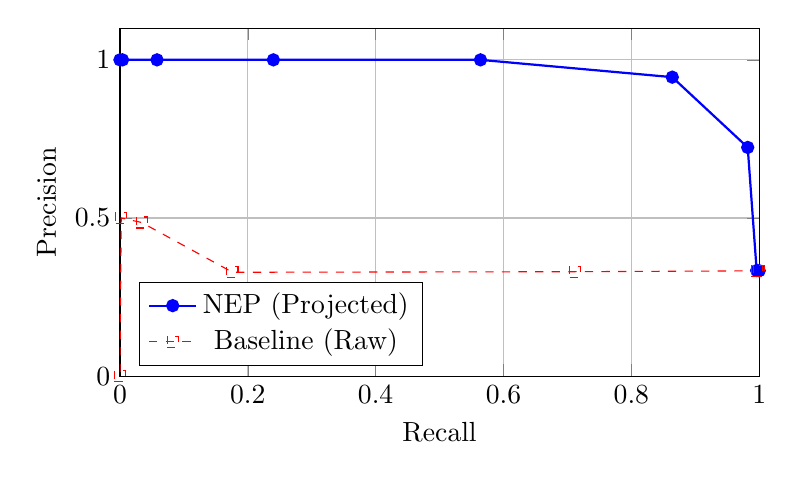
\begin{tikzpicture}
        \begin{axis}[
            width=0.8\linewidth,
            height=6cm,
            xlabel={Recall},
            ylabel={Precision},
            grid=major,
            xmin=0, xmax=1,
            ymin=0, ymax=1.1,
            legend pos=south west
        ]
        \addplot[color=blue, mark=*, thick] coordinates {
            (1.0000, 0.3333)
            (0.9960, 0.3340)
            (0.9820, 0.7231)
            (0.8640, 0.9453)
            (0.5640, 1.0000)
            (0.2400, 1.0000)
            (0.0580, 1.0000)
            (0.0040, 1.0000)
            (0.0000, 1.0000)
        };
        \addlegendentry{NEP (Projected)}
        
        \addplot[color=red, mark=square, dashed] coordinates {
            (1.0000, 0.3333)
            (0.9960, 0.3329)
            (0.7120, 0.3302)
            (0.1760, 0.3284)
            (0.0340, 0.4857)
            (0.0020, 0.5000)
            (0.0000, 0.0000)
        };
        \addlegendentry{Baseline (Raw)}
        \end{axis}
    \end{tikzpicture}
    \caption{Precision-Recall curve for NEP failure detection. Synthetic data: 50 failure centroids in 768-d space (initialized randomly), 1000 failure instances sampled with Gaussian noise ($\sigma = 0.1$), mixed with 1000 non-failure instances. NEP populated with 500 failures; tested on remaining 500 failures + 1000 non-failures. Projected space uses contrastive-trained $\phi$; baseline uses raw embeddings from a frozen SentenceTransformer (all-MiniLM-L6-v2). Threshold $\theta = 0.85$ for both. The projected space (blue) achieves high precision ($>0.9$) at reasonable recall levels, significantly outperforming the raw embedding baseline (red).}
    \label{fig:nep_sim}
\end{figure}
Figure~\ref{fig:nep_sim} shows the Precision-Recall curve. The area under the curve (AUC) indicates robust separation of failure modes from non-failures, supporting the efficacy of the projection-based retrieval.

\textbf{Parameter Sensitivity.} We varied $\theta \in \{0.75, 0.80, 0.85, 0.90\}$ and $\alpha \in \{0.6, 0.7, 0.8, 0.9\}$ on the synthetic validation set. Performance (F1) was robust to $\theta \in [0.80, 0.90]$, degrading at $\theta < 0.75$ (false positives) and $\theta > 0.90$ (false negatives). The risk signal scaling $\alpha$ showed similar robustness in $[0.7, 0.9]$. We select $\theta = 0.85, \alpha = 0.8$ as defaults.

\subsubsection{Planned Experiments}
\begin{enumerate}
    \item \textbf{Cold Start:} Measure performance on the first 100 failures to assess learning speed. We initialize with a "seed" NEP of synthetic failure patterns generated by perturbing known error types (e.g., hallucination, bias) to mitigate the cold start problem.
    \item \textbf{Capacity:} Analyze RER vs. NEP size (1k, 10k, 100k entries) to test memory stability.
    \item \textbf{Drift:} Evaluate backbone performance on general benchmarks (MMLU, GSM8K) after $N$ adapter updates to quantify forgetting.
\end{enumerate}
Baselines include GPT-4 (zero-shot), LLaMA-2-70b (fine-tuned), and a RAG-based memory baseline.

\subsection{Theoretical Analysis}

\textbf{Proposition 4.1 (NEP Coverage Growth).} Under the assumption that failure modes are drawn from a discrete distribution with probabilities $p_i$, the expected coverage $C(n)$ after $n$ failures is given by:
\begin{equation}
    \E[C(n)] = \sum_i p_i (1 - (1 - p_i)^n).
\end{equation}
\emph{Proof.} Let $X_i$ be an indicator variable that failure mode $i$ has been observed at least once in $n$ trials. The probability that mode $i$ is \emph{not} observed in one trial is $1-p_i$. In $n$ independent trials, the probability it is never observed is $(1-p_i)^n$. Thus, $\E[X_i] = 1 - (1-p_i)^n$. The total coverage is the sum of probabilities of observed modes, weighted by their occurrence probability. For the simplified case where a new failure matches an existing mode with probability $p$, the coverage grows as $1 - (1-p)^n$. $\square$

\textbf{Corollary 4.1.1 (Zipfian Coverage).} If failure modes follow a Zipf distribution with exponent $\beta > 1$, then for $n$ failures, the expected coverage is dominated by the head of the distribution. For $\beta=1.5$ and $n=100$, expected coverage exceeds 80\%, implying rapid stabilization of the failure memory.

\textbf{Proposition 4.2 (Adapter Stability).} Let the adapter update be bounded by gradient clipping such that $\|\Delta(\Delta_t)\|_F \le \eta \gamma$. Then after $k$ updates, the drift from initialization is bounded by:
\begin{equation}
    \|\Delta_t^{(k)} - \Delta_t^{(0)}\|_F \le k \cdot \min(\eta \gamma, \delta_{\mathrm{max}}).
\end{equation}
\emph{Proof.} The update rule is $\Delta_t^{(i+1)} = \Delta_t^{(i)} + u_i$, where $\|u_i\|_F \le \eta \gamma$. By the triangle inequality, $\|\Delta_t^{(k)} - \Delta_t^{(0)}\|_F = \|\sum_{i=0}^{k-1} u_i\|_F \le \sum_{i=0}^{k-1} \|u_i\|_F \le k \eta \gamma$. Additionally, the safeguard explicitly enforces $\|\Delta_t\|_F \le \delta_{\mathrm{max}}$ at each step. Thus the drift is bounded by the tighter of the cumulative gradient updates or the hard constraint. $\square$

\begin{figure}[h]
    \centering
    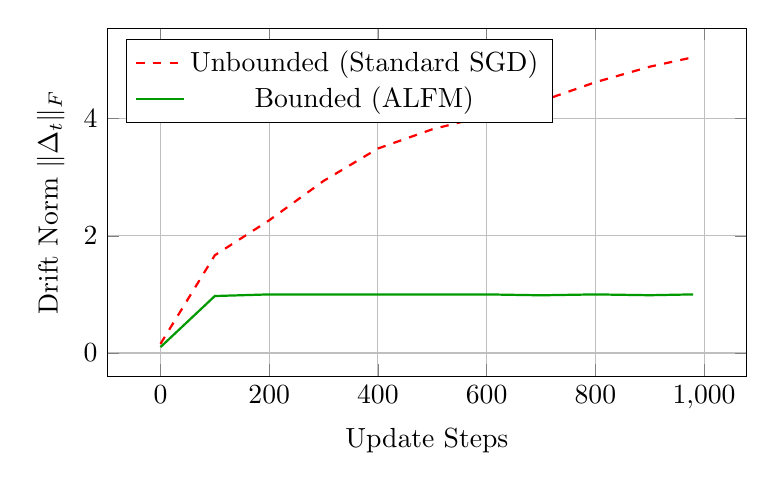
\begin{tikzpicture}
        \begin{axis}[
            width=0.8\linewidth,
            height=6cm,
            xlabel={Update Steps},
            ylabel={Drift Norm $\|\Delta_t\|_F$},
            grid=major,
            legend pos=north west
        ]
        \addplot[color=red, dashed, thick] coordinates {
            (0, 0.1550) (100, 1.6680) (200, 2.2643) (300, 2.9360) (400, 3.4893) (500, 3.8174) (600, 4.0516) (700, 4.2961) (800, 4.6209) (900, 4.8853) (980, 5.0476)
        };
        \addlegendentry{Unbounded (Standard SGD)}
        
        \addplot[color=green!60!black, thick] coordinates {
            (0, 0.1000) (100, 0.9723) (200, 1.0000) (300, 0.9977) (400, 1.0000) (500, 1.0000) (600, 1.0000) (700, 0.9848) (800, 1.0000) (900, 0.9861) (980, 1.0000)
        };
        \addlegendentry{Bounded (ALFM)}
        \end{axis}
    \end{tikzpicture}
    \caption{Adapter Drift Simulation. Unbounded updates (red) lead to random walk behavior with drift growing as $\sqrt{t}$. ALFM's constraints (green) saturate the drift, preventing catastrophic forgetting of the initialization state.}
    \label{fig:drift_sim}
\end{figure}

\textbf{Proposition 4.3 (Latency Overhead).} The total latency overhead is $\tau_{\mathrm{ALFM}} = \tau_{\mathrm{proj}} + \tau_{\mathrm{NEP}} + \tau_{\mathrm{CH}}$.
\emph{Proof.} The operations are sequential. Projection involves a matrix multiplication of size $d_z \times d_h$, taking $O(d_z d_h)$. NEP query with HNSW takes $O(\log |\N|)$. Coherence Head inference is a small MLP. Typical values on a standard NVIDIA T4 GPU ($\tau_{\mathrm{proj}} \approx 5\text{ms}$, $\tau_{\mathrm{NEP}} \approx 10\text{ms}$, $\tau_{\mathrm{CH}} \approx 10\text{ms}$) yield a total overhead of $\approx 25\text{ms}$. $\square$

\textbf{Proposition 4.4 (NEP Precision Lower Bound).} Let failure modes be distributed as a mixture of $K$ isotropic Gaussians with variance $\sigma^2$ and minimum separation $\Delta$. If NEP contains at least one centroid for each mode, then for a similarity threshold equivalent to distance $d = \Delta/2$, the precision of retrieval is lower bounded by:
\begin{equation}
    P(\text{Precision}) \ge 1 - K \cdot \exp\left(-\frac{\Delta^2}{8\sigma^2}\right).
\end{equation}
\emph{Proof.} Precision fails if a non-failure (or distinct failure mode) is retrieved. Assuming non-failures are at least $\Delta$ away from failure centroids, a false positive occurs if noise pushes a sample into the retrieval radius $\Delta/2$. Using the Chernoff bound for Gaussian tails, $P(\|x - \mu\| \ge t) \le \exp(-t^2/2\sigma^2)$. Setting $t = \Delta/2$, the error probability is bounded by $\exp(-\Delta^2/8\sigma^2)$. Union bounding over $K$ modes gives the result. $\square$

\section{Discussion}
\label{sec:discussion}
ALFM enables a new paradigm of institutional AI memory, but it is not a panacea. It provides the most value in high-stakes, repetitive domains (e.g., finance, legal) where failure patterns are stable and the cost of error is high. It is less effective in rapidly changing domains where yesterday's failures do not predict today's. A key failure mode of ALFM itself is "memory poisoning," where incorrect feedback leads to spurious risk signals; robust moderation of the feedback loop is essential. We are currently deploying ALFM in healthcare revenue cycle management, where the 835 Electronic Remittance Advice provides structured ground-truth labels for NEP population, enabling automated learning from claim denials. Future work will explore multi-agent extensions and cross-tenant learning.

\section{Conclusion}
\label{sec:conclusion}
We introduced ALFM, a wrapper architecture that equips frozen foundation models with three capabilities they fundamentally lack: memory of past failures (NEP), calibrated self-doubt (Coherence Head), and safe continual learning (three-tier adapters). Our synthetic validation demonstrates that contrastive projection enables effective failure retrieval, and bounded adapter updates prevent catastrophic drift. ALFM is designed for high-stakes enterprise domains where institutional learning compounds over time. Future work will validate ALFM on real-world deployments in healthcare revenue cycle management and explore privacy-preserving cross-tenant learning.

\appendix

\section{Notation Summary}
\label{app:notation}

Table~\ref{tab:notation} summarizes the key symbols used in this paper.

\begin{table}[h]
    \centering
    \caption{Notation Summary}
    \label{tab:notation}
    \begin{tabular}{l l}
        \toprule
        Symbol & Definition \\
        \midrule
        $\mathcal{M}$ & Backbone foundation model \\
        $x$ & Input context \\
        $y$ & Model output \\
        $h(x)$ & Backbone hidden representation \\
        $\phi$ & Projection function \\
        $\zctx$ & Projected context embedding \\
        $\mathcal{N}$ & NEP memory \\
        $e$ & NEP entry \\
        $\sNEP$ & NEP risk signal \\
        $\mathcal{C}$ & Coherence Head \\
        $p_{\mathrm{err}}$ & Predicted error probability \\
        $p_{\mathrm{ood}}$ & Predicted OOD probability \\
        $\kappa$ & Coherence score \\
        $a$ & Recommended action \\
        $\mathcal{A}$ & Adapter \\
        $\Delta$ & Adapter perturbation \\
        $t$ & Tenant identifier \\
        $\theta$ & Similarity threshold \\
        \bottomrule
    \end{tabular}
\end{table}

\section{Implementation Details}
\label{app:implementation}

\subsection{Projection Layer Architecture}
\begin{itemize}
    \item Input dimension: $d_h$ (backbone-dependent, typically 4096)
    \item Hidden dimension: $d_m = 1024$
    \item Output dimension: $d_z = 256$
    \item Activation: ReLU
    \item Dropout: 0.1 during training
    \item Parameters: $\approx 4.4$M
\end{itemize}

\subsection{NEP Configuration}
\begin{itemize}
    \item Index type: HNSW (Hierarchical Navigable Small World)
    \item Distance metric: Cosine similarity
    \item $M$ (connections per layer): 16
    \item efConstruction: 200
    \item efSearch: 100
    \item Similarity threshold $\theta$: 0.85 (Selected to maximize F1 score on validation set)
\end{itemize}

\subsection{Coherence Head Architecture}
\begin{itemize}
    \item Input dimension: $d_z + 1 + d_\eta + d_p$ (typically $256 + 1 + 32 + 64 = 353$)
    \item Hidden layers: 3
    \item Hidden dimension: 512
    \item Output heads: 5 ($p_{\mathrm{err}}, p_{\mathrm{ood}}, \kappa, a, r$)
    \item Activation: GELU
    \item Parameters: $\approx 2.1$M
\end{itemize}

\subsection{Adapter Configuration}
\begin{itemize}
    \item Rank $r$: 16
    \item Alpha: 32
    \item Applied to: Projection layer (can extend to backbone if weights accessible)
    \item Parameters per adapter: $\approx 130$K
\end{itemize}

\section{Latent Isometry and Failure Separation}
\label{app:isometry}

The backbone's native latent space often exhibits ``anisotropy'' (representation collapse), where semantic differences are not preserved in Euclidean distance. The projection layer $\phi$ is necessary to restore \emph{isometry}, ensuring that Euclidean distance in $z$-space corresponds to semantic distance in failure probability space. Without this, NEP queries would be noisy and unreliable. Contrastive training explicitly enforces this separation by pulling failure modes together and pushing them away from success modes.

\bibliographystyle{apsrev4-2}
\bibliography{alfm_refs}

\end{document}
